%%%%%%%%%%%%%%%%%%%%%%%%%%%%%%%%%%%%%%%%%
% baposter Landscape Poster
% LaTeX Template
% Version 1.0 (11/06/13)
%
% baposter Class Created by:
% Brian Amberg (baposter@brian-amberg.de)
%
% This template has been downloaded from:
% http://www.LaTeXTemplates.com
%
% License:
% CC BY-NC-SA 3.0 (http://creativecommons.org/licenses/by-nc-sa/3.0/)
%
%%%%%%%%%%%%%%%%%%%%%%%%%%%%%%%%%%%%%%%%%

%----------------------------------------------------------------------------------------
%	PACKAGES AND OTHER DOCUMENT CONFIGURATIONS
%----------------------------------------------------------------------------------------

\documentclass[landscape,a0paper,fontscale=0.375]{baposter} % Adjust the font scale/size here (fontscale=0.285)

\usepackage{graphicx} % Required for including images
\graphicspath{{figures/}} % Directory in which figures are stored

\usepackage{amsmath} % For typesetting math
\usepackage{amssymb} % Adds new symbols to be used in math mode

\usepackage{booktabs} % Top and bottom rules for tables
\usepackage{enumitem} % Used to reduce itemize/enumerate spacing
\usepackage{palatino} % Use the Palatino font
\usepackage[font=small,labelfont=bf]{caption} % Required for specifying captions to tables and figures

\usepackage{multicol} % Required for multiple columns
\setlength{\columnsep}{1.5em} % Slightly increase the space between columns
\setlength{\columnseprule}{0mm} % No horizontal rule between columns

\usepackage{xcolor} % color in RGB

\usepackage{tikz} % Required for flow chart
\usetikzlibrary{shapes,arrows} % Tikz libraries required for the flow chart in the template

%\usepackage{etex}			%%%%% bib setup from our main
%\usepackage{etoolbox}
%\usepackage{keyval}
%\usepackage{ifthen}
%\usepackage{url}
%\usepackage{csquotes}
%\usepackage[backend=biber, url=true, doi=true, style=numeric, sorting=none]{biblatex}

\newcommand{\compresslist}{ % Define a command to reduce spacing within itemize/enumerate environments, this is used right after \begin{itemize} or \begin{enumerate}
\setlength{\itemsep}{1pt}
\setlength{\parskip}{0pt}
\setlength{\parsep}{0pt}
}

%\definecolor{lightblue}{RGB}{33,26,82} % Defines the color used for content box headers
\definecolor{lightblue}{rgb}{0.145,0.6666,1} % Defines the color used for content box headers
\definecolor{aaublue}{rgb}{0.1294117647,0.1019607843,0.3215686275}  %<--define aaublue

\begin{document}

\begin{poster}
{
headerborder=closed, % Adds a border around the header of content boxes
colspacing=1em, % Column spacing
bgColorOne=white, % Background color for the gradient on the left side of the poster
bgColorTwo=white, % Background color for the gradient on the right side of the poster
borderColor=lightblue, % Border color
headerColorOne=aaublue, % Background color for the header in the content boxes (left side)
headerColorTwo=lightblue, % Background color for the header in the content boxes (right side)
headerFontColor=white, % Text color for the header text in the content boxes
boxColorOne=white, % Background color of the content boxes
textborder=roundedleft, % Format of the border around content boxes, can be: none, bars, coils, triangles, rectangle, rounded, roundedsmall, roundedright or faded
eyecatcher=true, % Set to false for ignoring the left logo in the title and move the title left
headerheight=0.1\textheight, % Height of the header
headershape=roundedright, % Specify the rounded corner in the content box headers, can be: rectangle, small-rounded, roundedright, roundedleft or rounded
headerfont=\Large\bf\textsc, % Large, bold and sans serif font in the headers of content boxes
%textfont={\setlength{\parindent}{1.5em}}, % Uncomment for paragraph indentation
linewidth=2pt % Width of the border lines around content boxes
}
%----------------------------------------------------------------------------------------
%	TITLE SECTION 
%----------------------------------------------------------------------------------------
%
{
\includegraphics[height=2.7em]{group7404.png}} % First university/lab logo on the left
{\bf \fontsize{1.5cm}{1.5cm} THE \hspace{3pt} EFFECT \hspace{3pt} OF \hspace{3pt} LIMB \hspace{3pt} POSITION \hspace{3pt} ON \hspace{3pt} MYOELECTRIC \hspace{3pt} PROSTHETIC \hspace{3pt} CONTROL\\ \vspace{0.2em} USING \hspace{3pt} LINEAR \hspace{3pt} REGRESSION \vspace{0.5em}} % Poster title %The effect of limb position on myoelectric prosthetic control using linear regression 
{\ \textit{Irene Uriarte, Martin Garenfeld, Oliver Damsgaard, Simon Bruun.} Aalborg University, School of Medicine and Health \vspace{0.05em}} % Author names and institution
{
\includegraphics[height=7em]{AAU_LOGO_RGB_UK.png}} % Second university/lab logo on the right

%----------------------------------------------------------------------------------------
%	INTRODUCTION
%----------------------------------------------------------------------------------------

\headerbox{Introduction}{name=introduction,column=0,row=0}{
	
	%The development of EMG controlled prosthetics have advanced greatly in recent years. More complex prosthetics are demanded and more advanced control mothods has been developed. Most control methods so far has utilized pattern recognition which only enables control of one degree of freedom at a time. Most studies have conducted tests in only one limb position, not considering the limb position effect on EMG signals. \cite{Fougner2011} This study aims to overcome the limb position effect by combining EMG with inertial information in the training sessions of the regressor to obtain simultaneous and proportional control of EMG prosthesis.
	Electromyography (EMG) is widely used for controlling functional prosthetics. However, EMG signals for the same movements change with variations in limb position and lowers the accuracy in control schemes \cite{Fougner2011}. Most previous studies have utilized classification for pattern recognition when changing limb position, with a negative effect in performance. Linear regression is a newer method in control of myoelectric prosthetics, which has proven to yield robust simultaneous and proportional control \cite{hahne2014}. Only the RMS feature was previously tested in variations of limb positions in regression-based control \cite{Hwang2017}. This study investigated the effect of limb position in a linear regression-based control scheme, when using the commonly used Mean Absolute Value (MAV) and Logarithmic Variance (LogVar) feature, where the latter has shown linear properties \cite{hahne2014}.
}

%----------------------------------------------------------------------------------------
%	OBJECTIVES   bottomaligned=objectives
%----------------------------------------------------------------------------------------

\headerbox{Aim}{name=aim,column=1,row=0}{

The aim for this project is expressed in the following hypothesis:

%hypotheses
\begin{itemize}
	\item It is possible to yield similar performance in different limb positions in myoelectric prosthetic control using a linear regression based control scheme.
\end{itemize}

\vspace{0.3em} % When there are two boxes, some whitespace may need to be added if the one on the right has more content
}

%----------------------------------------------------------------------------------------
%	RESULTS 1	Offline training results
%----------------------------------------------------------------------------------------

\headerbox{Offline Results}{name=results,column=2,span=2,row=0}{
	
	
\begin{multicols}{2}
	
	\begin{center}
		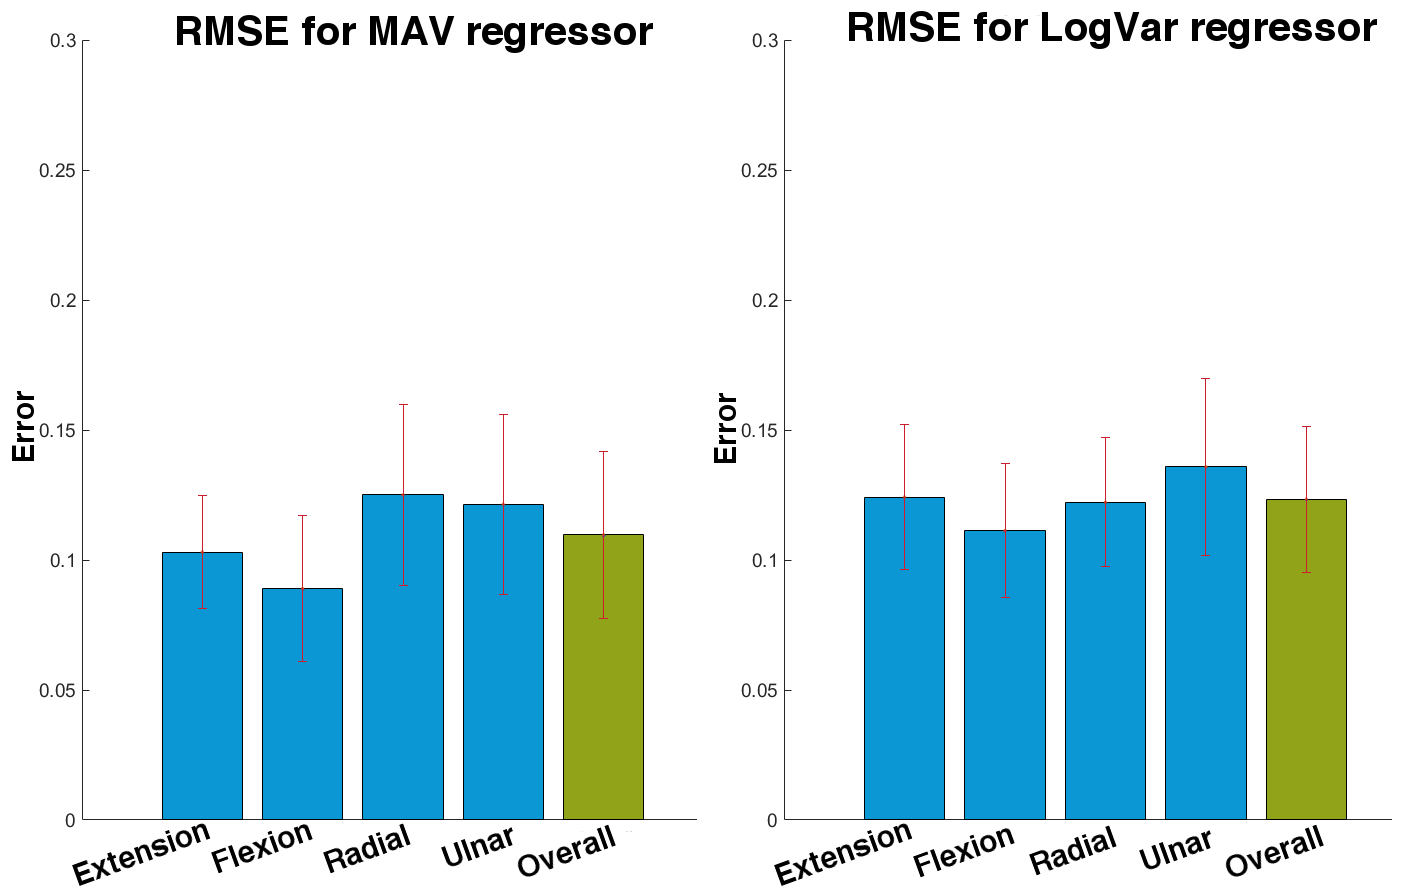
\includegraphics[width=1\linewidth]{gimmeThemRMSEBars}
		\captionof*{figure}{\textbf{Figure 2:} RMSE when using training data.}
	\end{center}
	
	Comparing the RMSE of MAV and LogVar through a Friedman's test indicates a significant difference (p = 0.0007), where LogVar has the higher mean. 
	
	\begin{center}
		\begin{tabular}{l l l}
			\toprule
			\textbf{Feature} & \textbf{Overall mean error} & \textbf{Standard deviation}\\
			\midrule
			MAV & 0.1096 &  $\pm 0.0321$ \\
			LogVar & 0.1234 & $\pm 0.0281$ \\
			\bottomrule
		\end{tabular}
		\captionof{table}{Overall mean RMSE when using training data as input in the regression model}
	\end{center}
	
\begin{center}
	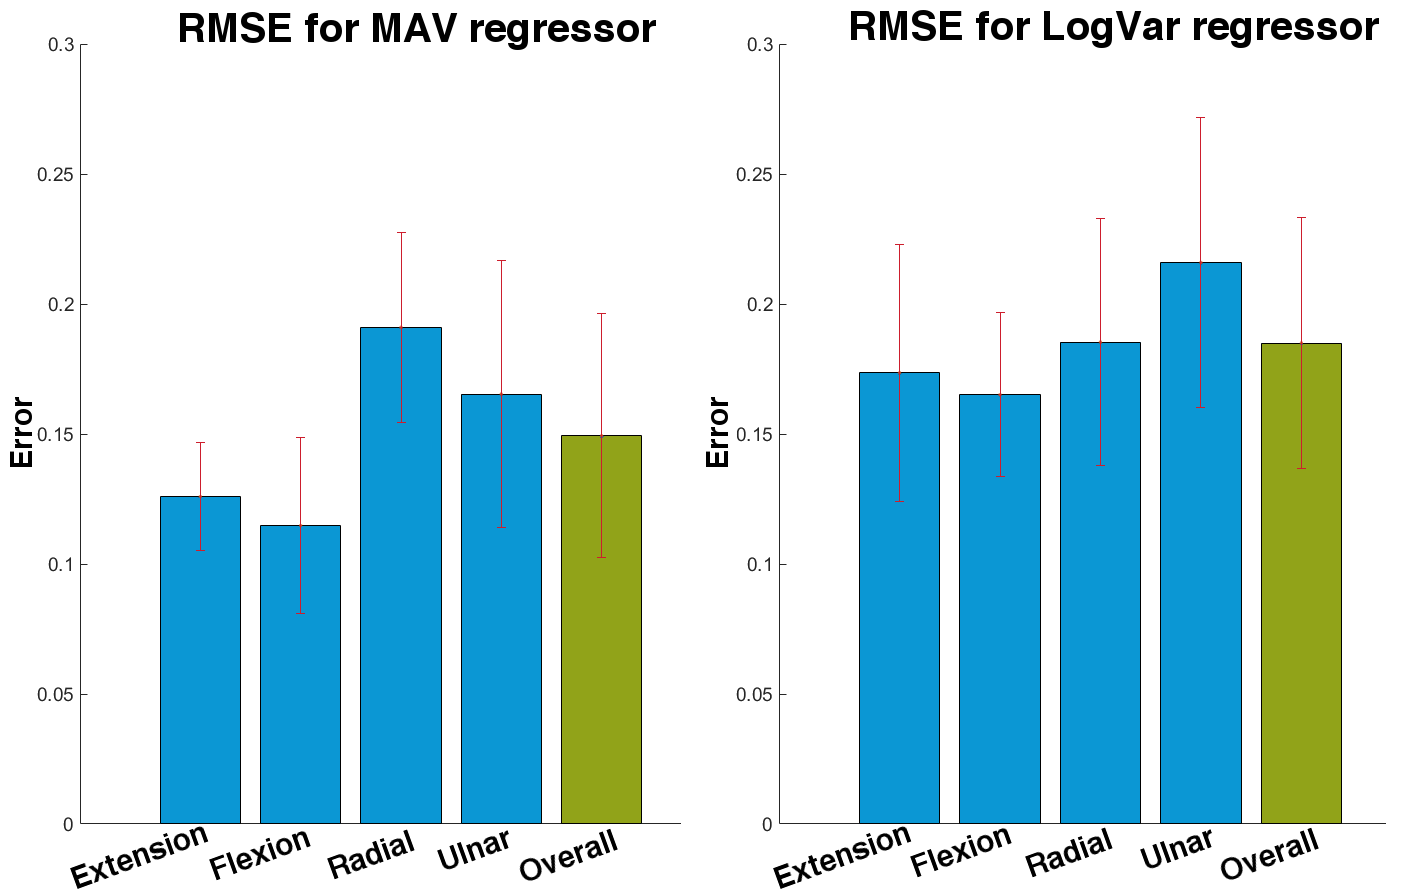
\includegraphics[width=1\linewidth]{RMSEBarPlotNewData}
	\captionof*{figure}{\textbf{Figure 3:} RMSE when using test data}
\end{center}
	
	\begin{center}
		\begin{tabular}{l l l}
			\toprule
			\textbf{Feature} & \textbf{Overall mean error} & \textbf{Standard deviation}\\
			\midrule
			MAV & 0.1493 & $\pm 0.0469$ \\
			LogVar & 0.1850 & $\pm 0.0484$ \\
			\bottomrule
		\end{tabular}
		\captionof{table}{Overall mean RMSE when using test data as input in the regression model}
	\end{center}

Comparing the RMSE of MAV and LogVar when using test data again indicated significant difference (p = 0.0082), where LogVar again has the higher mean. The RMSE of the MAV when using training data proves significantly smaller than the RMSE when using test data (p = 0.0002). Similar results are obtained for the LogVar regressor (p = 0.0002).

\end{multicols}
\vspace{1em}


%%------------------------------------------------
%
%\begin{multicols}{2}
%
%\begin{center}
%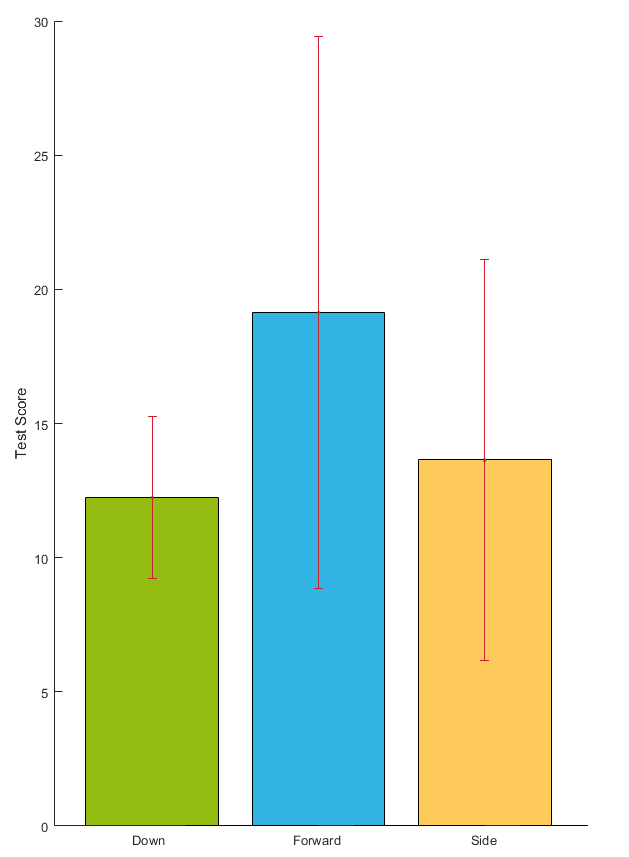
\includegraphics[width=0.2\linewidth]{TestScore}
%\captionof{figure}{The mean test score among four subjects when using regressors trained with Log-Var including IMU information}
%\end{center}
% 
%text?
%\end{multicols}
}

%----------------------------------------------------------------------------------------
%	REFERENCES
%----------------------------------------------------------------------------------------

\headerbox{References}{name=references,column=1,span=2,above=bottom}{

\renewcommand{\section}[2]{\vskip 0.05em} % Get rid of the default "References" section title
\nocite{*} % Insert publications even if they are not cited in the poster
\small{ % Reduce the font size in this block
\bibliographystyle{unsrt}
\bibliography{sample} %%% MANUALLY ADD SOURCES FROM THE MAIN.BIB TO THE SAMPLE.BIB !!!
}}

%----------------------------------------------------------------------------------------
%	FUTURE RESEARCH
%----------------------------------------------------------------------------------------
%
%\headerbox{Future Research}{name=futureresearch,column=1,span=2,aligned=references,above=bottom}{ % This block is as tall as the references block
%
%\begin{multicols}{2}
%Integer sed lectus vel mauris euismod suscipit. Praesent a est a est ultricies pellentesque. Donec tincidunt, nunc in feugiat varius, lectus lectus auctor lorem, egestas molestie risus erat ut nibh.
%
%Maecenas viverra ligula a risus blandit vel tincidunt est adipiscing. Suspendisse mollis iaculis sem, in \emph{imperdiet} orci porta vitae. Quisque id dui sed ante sollicitudin sagittis.
%\end{multicols}
%}

%----------------------------------------------------------------------------------------
%	CONTACT INFORMATION
%----------------------------------------------------------------------------------------

\headerbox{Acknowledgement}{name=contact,column=3,aligned=references,above=bottom}{ % This block is as tall as the references block

We would like to thank our supervisors Strahinja Dosen, Jakob Lund Dideriksen and Lotte N.S. Andreasen Struijk, and the School of Medicine and Health for providing equipment. Also a thanks to the test subjects who participated.%, with an extra applaud to Mikkel Birkedal for his dedication. 

}

%----------------------------------------------------------------------------------------
%	CONCLUSION
%----------------------------------------------------------------------------------------

\headerbox{Discussion}{name=conclusion,column=2,span=2,row=0,below=results,above=references}{

\begin{multicols}{2}
	
\begin{itemize}
	
	\item The online test results indicate that linear regression can be implemented as control scheme in myoelectric prosthetic control to yield similar performance across variations of limb position. This is opposed to previous studies using classification as control scheme.
	\item It was found that offline and online performance of the implemented regressors is not necessarily correlated. The offline tests showed overfitting of the regression models, but the online test yielded robust control of wrist movements in all limb positions, which could be a result of the subjects$'$ ability to compensate for a poorer fitting model, when visual feedback is provided. \vspace{2cm} 
	
	
	\item Even though LogVar shows linear properties in previous studies, the online test show no significant difference in performance when compared to MAV. 
	\item Linear regression has the potential to be used in future control schemes for myoelectric prosthetics for use in daily life tasks. 
	
\end{itemize}

\end{multicols}
}

%----------------------------------------------------------------------------------------
%	MATERIALS AND METHODS
%----------------------------------------------------------------------------------------

\headerbox{Methods and Material}{name=method,column=0,below=introduction,bottomaligned=references}{ % This block's bottom aligns with the bottom of the conclusion block

Surface EMG (sEMG) data was collected from seven able-bodied subjects. The subjects were instructed to performed four different hand gestures (flexion, extension, radial deviation and ulnar deviation), in three limb positions (down the side, lifted to the side, lifted forward). sEMG signals were recorded with a Myo armband (eight channels, 200Hz sample rate), positioned on the dominant forearm of the subjects while standing.

%The sEMG was recorded from eight channels with a 200Hz sample rate. Filtering was done with a second-order Butterworth high-pass filter ($f_c$ = 10Hz). 
%
%Features were extracted using a window of 40 samples with 50\% overlap. 
%MAV represent the amplitude of the signal. It is defined as the average of the absolute values of the sEMG signal:
%\vspace{-0.2cm}
%\begin{equation}
%MAV = \frac{1}{N}\sum\limits_{i=1}^N|x_i|
%\end{equation} \vspace{-0.1cm}
%
%where N is the length of the signal, and $x_i$ is the signal of $i$ samples.
%LogVar is a nonlinear transformation of the variance: %applied to %linealidad
%\vspace{-0.2cm}
%\begin{equation} \label{eq:logvar}
%log(\sigma^2) = log(\frac{\sum\limits_{i=1}^N(x_i - \mu)^2}{N})
%\end{equation}\vspace{-0.3cm}
%
%where $N$ is the length of the signal, $x_i$ is the $i^{th}$ sample of the signal and $\mu$ is the mean.
%PCA is applied to qualitatively determine the separability of the feature data. %Data is evaluated for differncies in feature data clusters and significant outliers. If the feature clusters are distinguishable from each other and have no significant outliers, the data is of high quality and will be used to train the regressors. Only the first three principal components identified through PCA will be used to train the regressors.
The regression models (regressors) were calculated as following:
\vspace{-0.1cm}
\begin{equation} \label{eq:simpleLinearRegression}
Y = \alpha + \beta X
\end{equation} \vspace{-0.7cm}

%where $Y$ is the estimated output, $X$ is the extracted feature data, $\beta$ is the regression coefficient, and $\alpha$ is the Y intercept.

One regressor was build for each wrist movement for each test subject: four for each feature. The offline regressor accuracy was tested qualitatively through superimposition of the output of the regressors build for each feature onto the actual data. The regressors were tested quantitatively by calculating the Root Mean Square Error (RMSE) between the expected movement and the regressor output. This was done for both training and test data to evaluate if the regressor had over- or under-fitted to the training data. 
As an alternative to testing the regressors with an actual prosthesis, the regressors were tested online in a virtual environment, where the time to complete a target-reaching task of 16 targets was measured. 

\begin{center}
	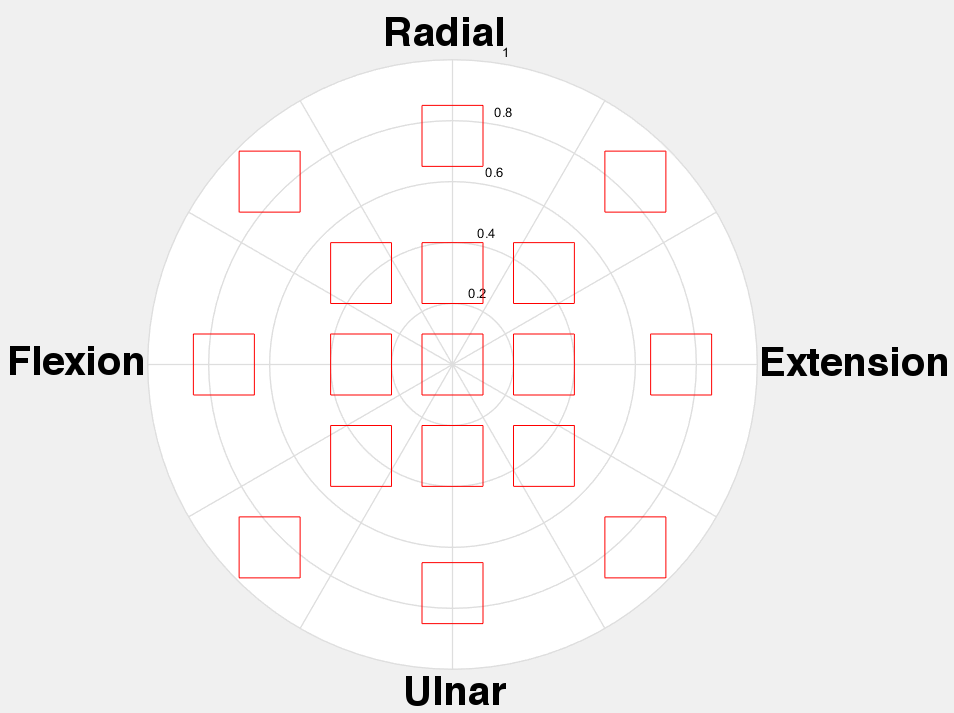
\includegraphics[width=0.8\linewidth]{NewPlacesToGo.png}
	\captionof*{figure}{\textbf{Figure 1:} The interface for the target reaching task. During testing an arrow originating from origin would show direction and intensity of movement.}
\end{center} \vspace{-0.3cm}

The performance (time per reached target) of the online test was compared between the different limb positions of the same feature and between all limb positions of the two features through statistical analysis.
%\vspace{0.5cm}
}

%----------------------------------------------------------------------------------------
%	RESULTS 2 Online training results
%----------------------------------------------------------------------------------------

\headerbox{Online Results}{name=results2,column=1,below=aim,bottomaligned=conclusion}{ % This block's bottom aligns with the bottom of the conclusion block
	
Results for the online test of regressor accuracy and control. The test is performed in a modified Fitts' Law test of reaching targets. The score is calculated as time per reached targets.

\vspace{-0.4cm}
\begin{center}
	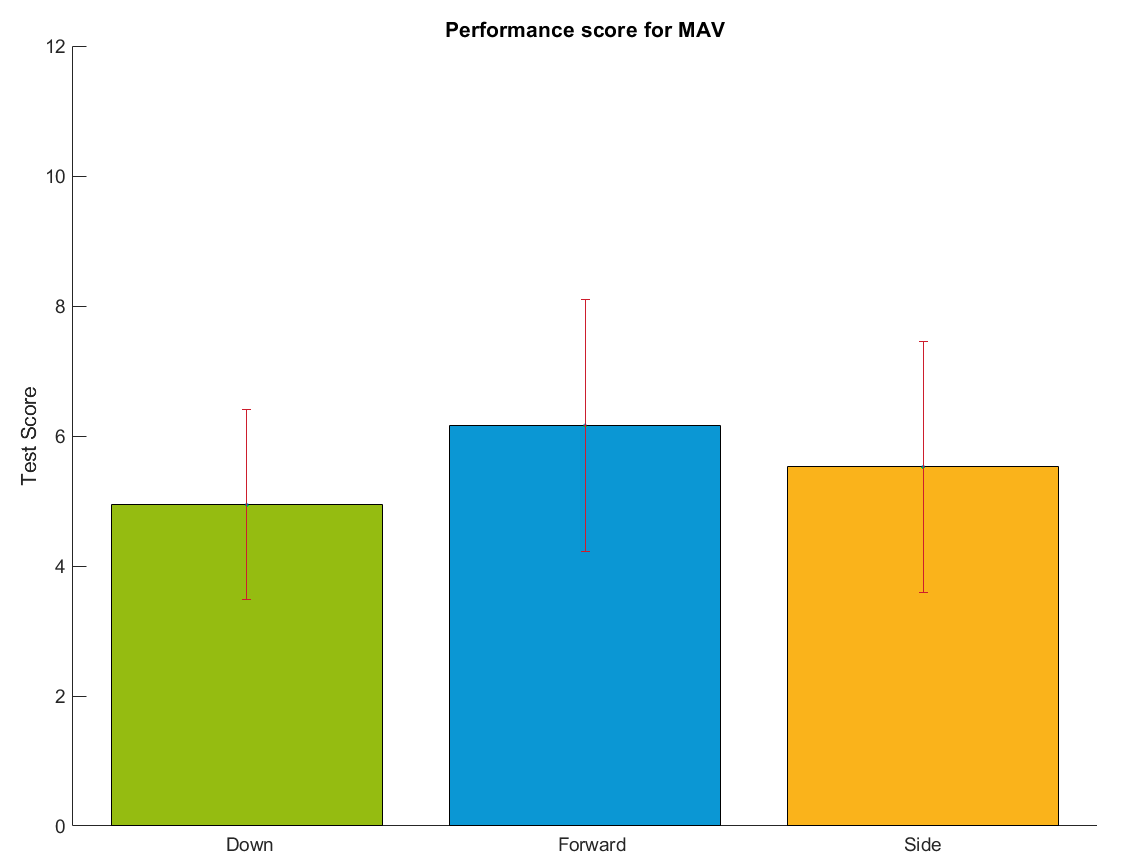
\includegraphics[width=0.7\linewidth]{gotItMAV}
	\captionof*{figure}{\textbf{Figure 4:} The mean test score among seven subjects when using regressors trained with MAV}
\end{center}

\vspace{-0.6cm}
\begin{center}
	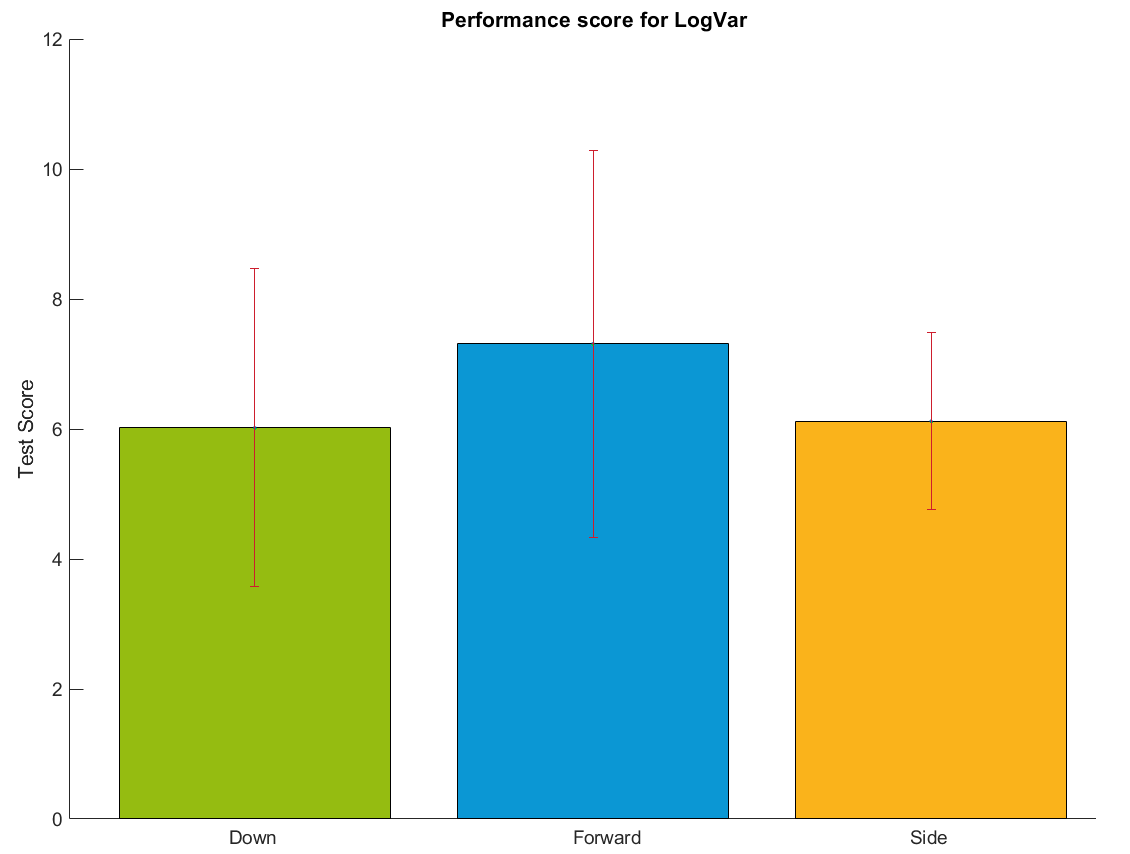
\includegraphics[width=0.7\linewidth]{gotItLogVar}
	\captionof*{figure}{\textbf{Figure 5:} The mean test score among seven subjects when using regressors trained with LogVar}
\end{center}
	
Using a Friedman's test the performance scores between the three limb positions prove not to be significantly different (p = 0.1561), when applying the MAV trained regressors in the online test. For the LogVar trained regressors the performance score between all limb positions cannot be proven significantly different either (p = 0.5647). There was no significant difference in the time to reach the targets across the two features (MAV: 5.5 s, LogVar: 6.5 s; p = 0.13).

}

%----------------------------------------------------------------------------------------

\end{poster}

\end{document}